\chapter{Modelling Larval Stage in a Vial}
Competition for food during the larval stage is determined by not only larval density but also ecological factors inside a food vial such as nitrogenous waste build-up, diffusion of waste in the food below, total food amount \citep{sarangiEcologicalDetailsMediate2018}. Thus, in order to investigate the adaptation to larval crowding, it is crucial to understand the ecology of a vial in which the larval stage of Drosophila lab populations is maintained and replicating such environment during larval feeding becomes the first step in modelling the larval growth. Previous experimental studies on Drosophila in laboratory conditions have shown the pattern of the growth of larvae, excretion of nitrogenous waste, larval feeding behaviour in response to the various levels of larval crowding \citep{sarangiEcologicalDetailsMediate2018}. Based on these experimental studies, I have created an individual-based model which considers larval trait parameters such as - feeding rate, efficiency to convert food into biomass, critical size and waste tolerance, to measure other traits like larval body size, development time, and survivorship.
\section{Ecology of a Culture Vial}
During larval feeding inside a vial, larvae can access only a certain amount of food from the total food available at a given time point. This is due to their inability to dig more to access food, and this accessible part of the food is referred as the feeding band \citep{godoy-herreraInterIntrapopulationalVariation1977,sarangiEcologicalDetailsMediate2018}. For simplicity, feeding band is taken as volume of food proportional to the width of the vial. In the model, I also assume this feeding band to be a constant volume of food in all types of culture vials till it reaches the bottom of the vial (In LCU culture vials, fedding band is smaller). In the model, the growth of larvae is affected by waste build-up and food quality in the feedin band. I also consider a diffusion band which is a part of the total food below feeding band where some amount of waste can diffuse from feeding band at each time step. Fig~\ref{fig:vial} is the visualization of feeding band and diffusion band during larval feeding.

\begin{figure}[h]
  \centering
  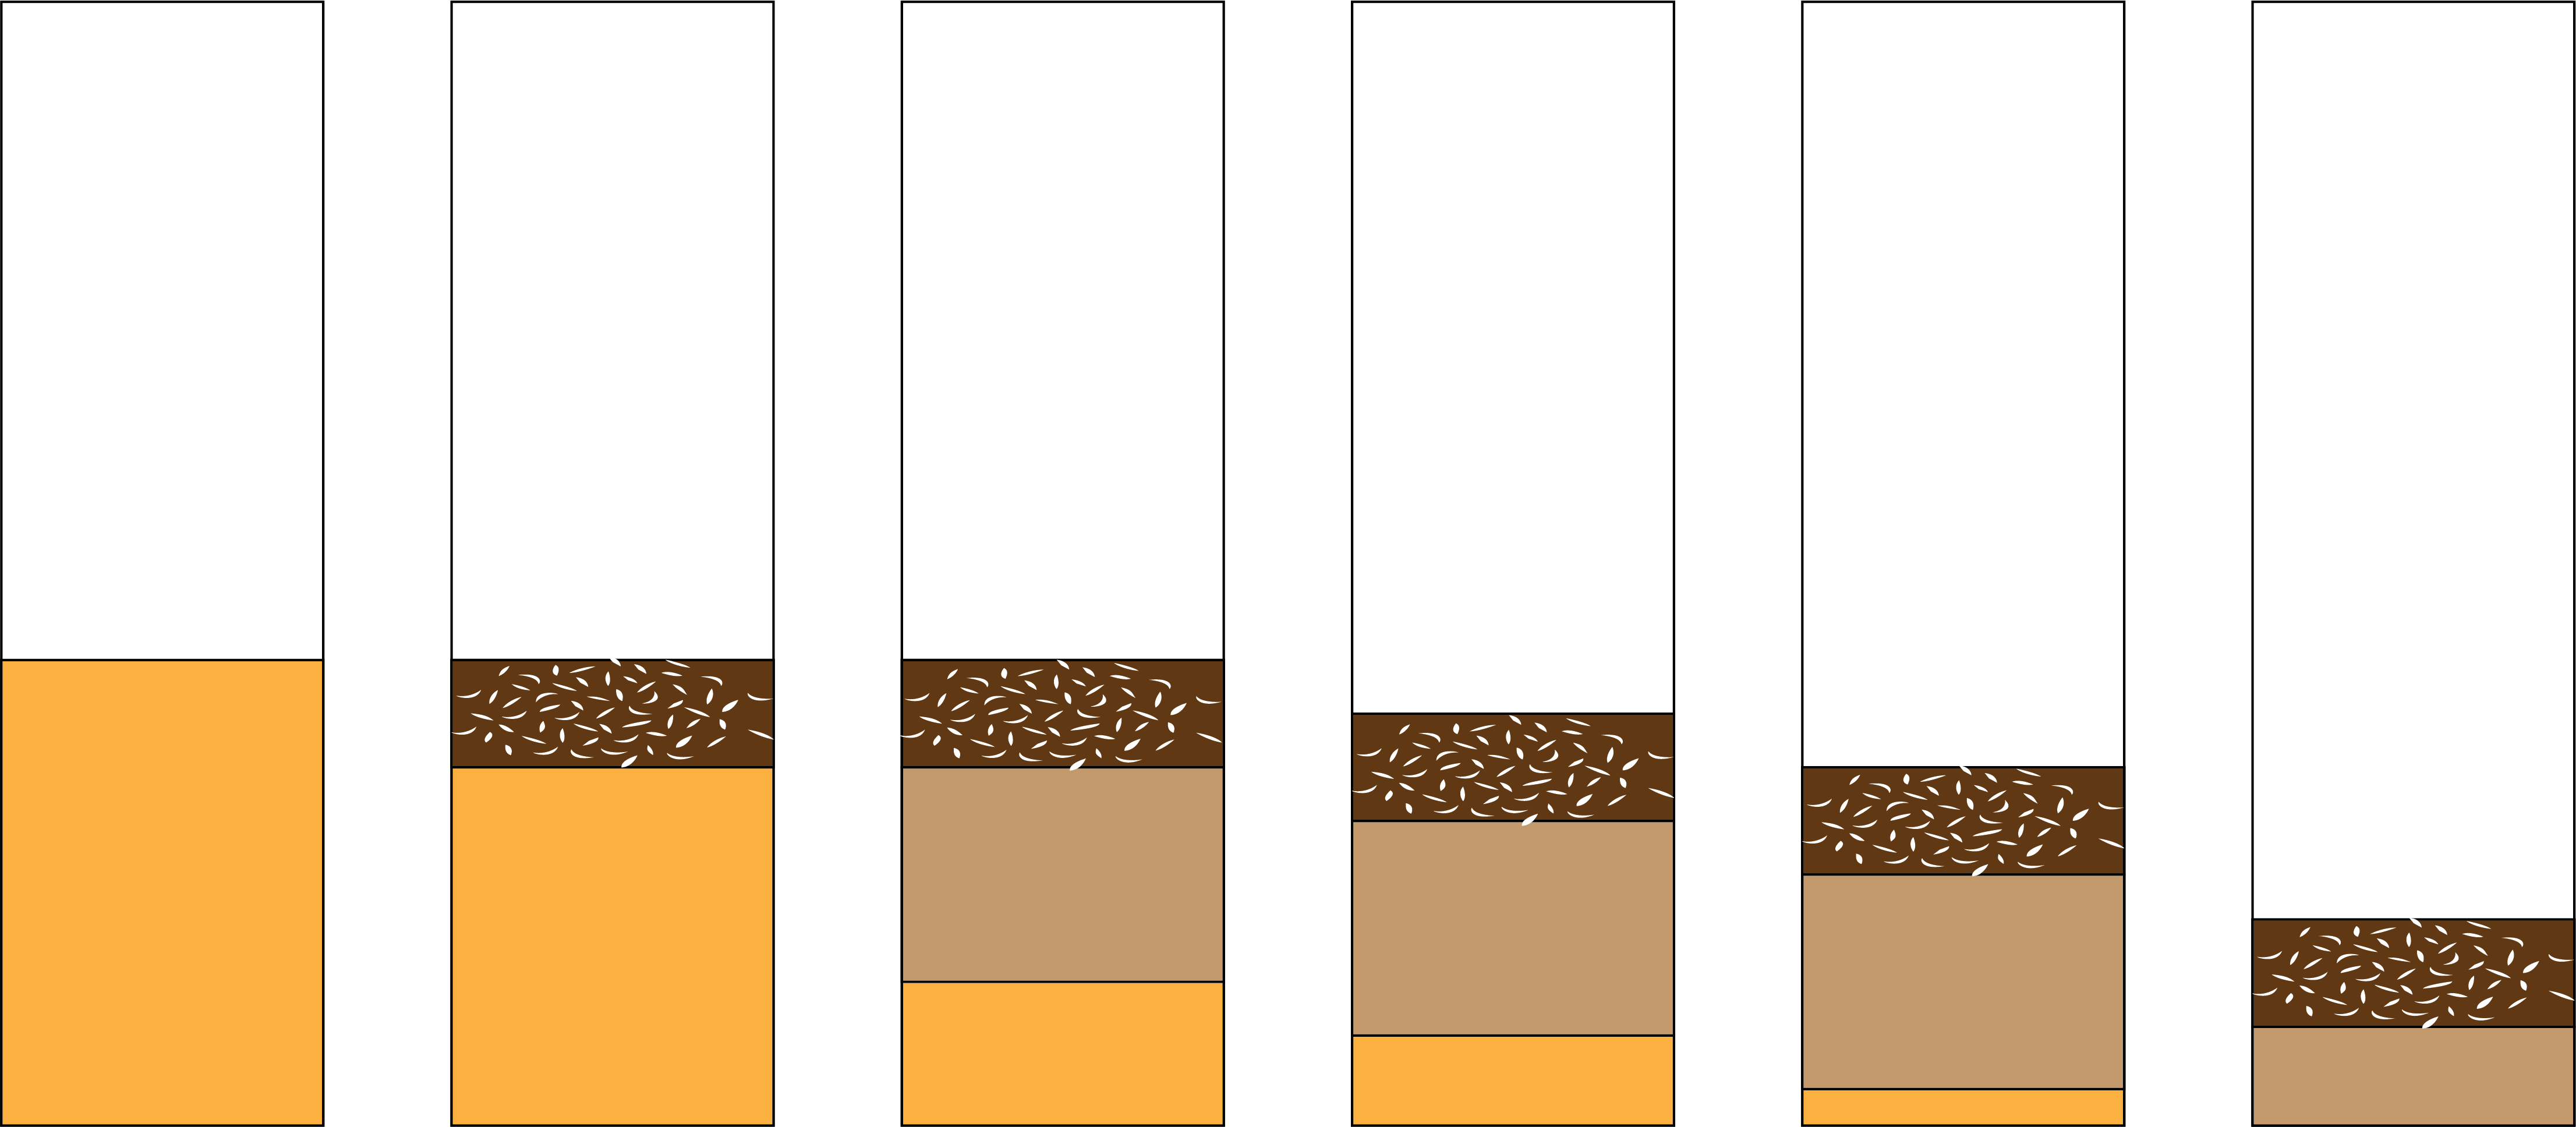
\includegraphics[width=0.75\textwidth]{C2/Figs/vial_diagram.png}
  \caption{Ecological dynamics in a vial during larval feeding}
  \label{fig:vial}
\end{figure}

\section{Larval Stage Model}
Each individual egg is assigned larval trait parameters from respective distributions with certain mean and variation given in table~\ref{tab:trait_value}. For a given amount of food and number of eggs, the model follows certain set of rules as described in fig~\ref{fig:larval_model} which are simulated in discrete time steps. The sex ratio within eggs is kept 1:1. Critical size and efficiency are taken as sexually dimorphic traits and are assigned depending on the sex of the individual larva. Critical size and efficiency of females are assumed to be 20\% higher than that of males, so that females attain higher body size in the same time period as males but survivorship between sexes is same. \citep{joshiGeneticsLarvalUrea1996,testaSexSpecificWeightLoss2013}\\ \\
The inital size of all larvae is same and the growth is determined by larval trait parameters such as initial feeding rate, efficiency, waste tolerance and critical size. The larval growth is divided into two stages determined by whether critical size is reached or not, These stages are called pre-critical and post-critical stage. \\
In pre-critical stage of the larva, feeding rate is a linear function of time, given as:
\[Fr_{i}(t) = fr_{i} + x_{1}\cdot t\]
Here, \\
$fr_{i}$: initial feeding rate of $i^{th}$ larva; \\
$x_{1}$: scaling parameter, \\
$t$: given time step; \\
$Fr_{i}(t)$: feeding rate at time $t$\\
\begin{figure}[h]
  \centering
  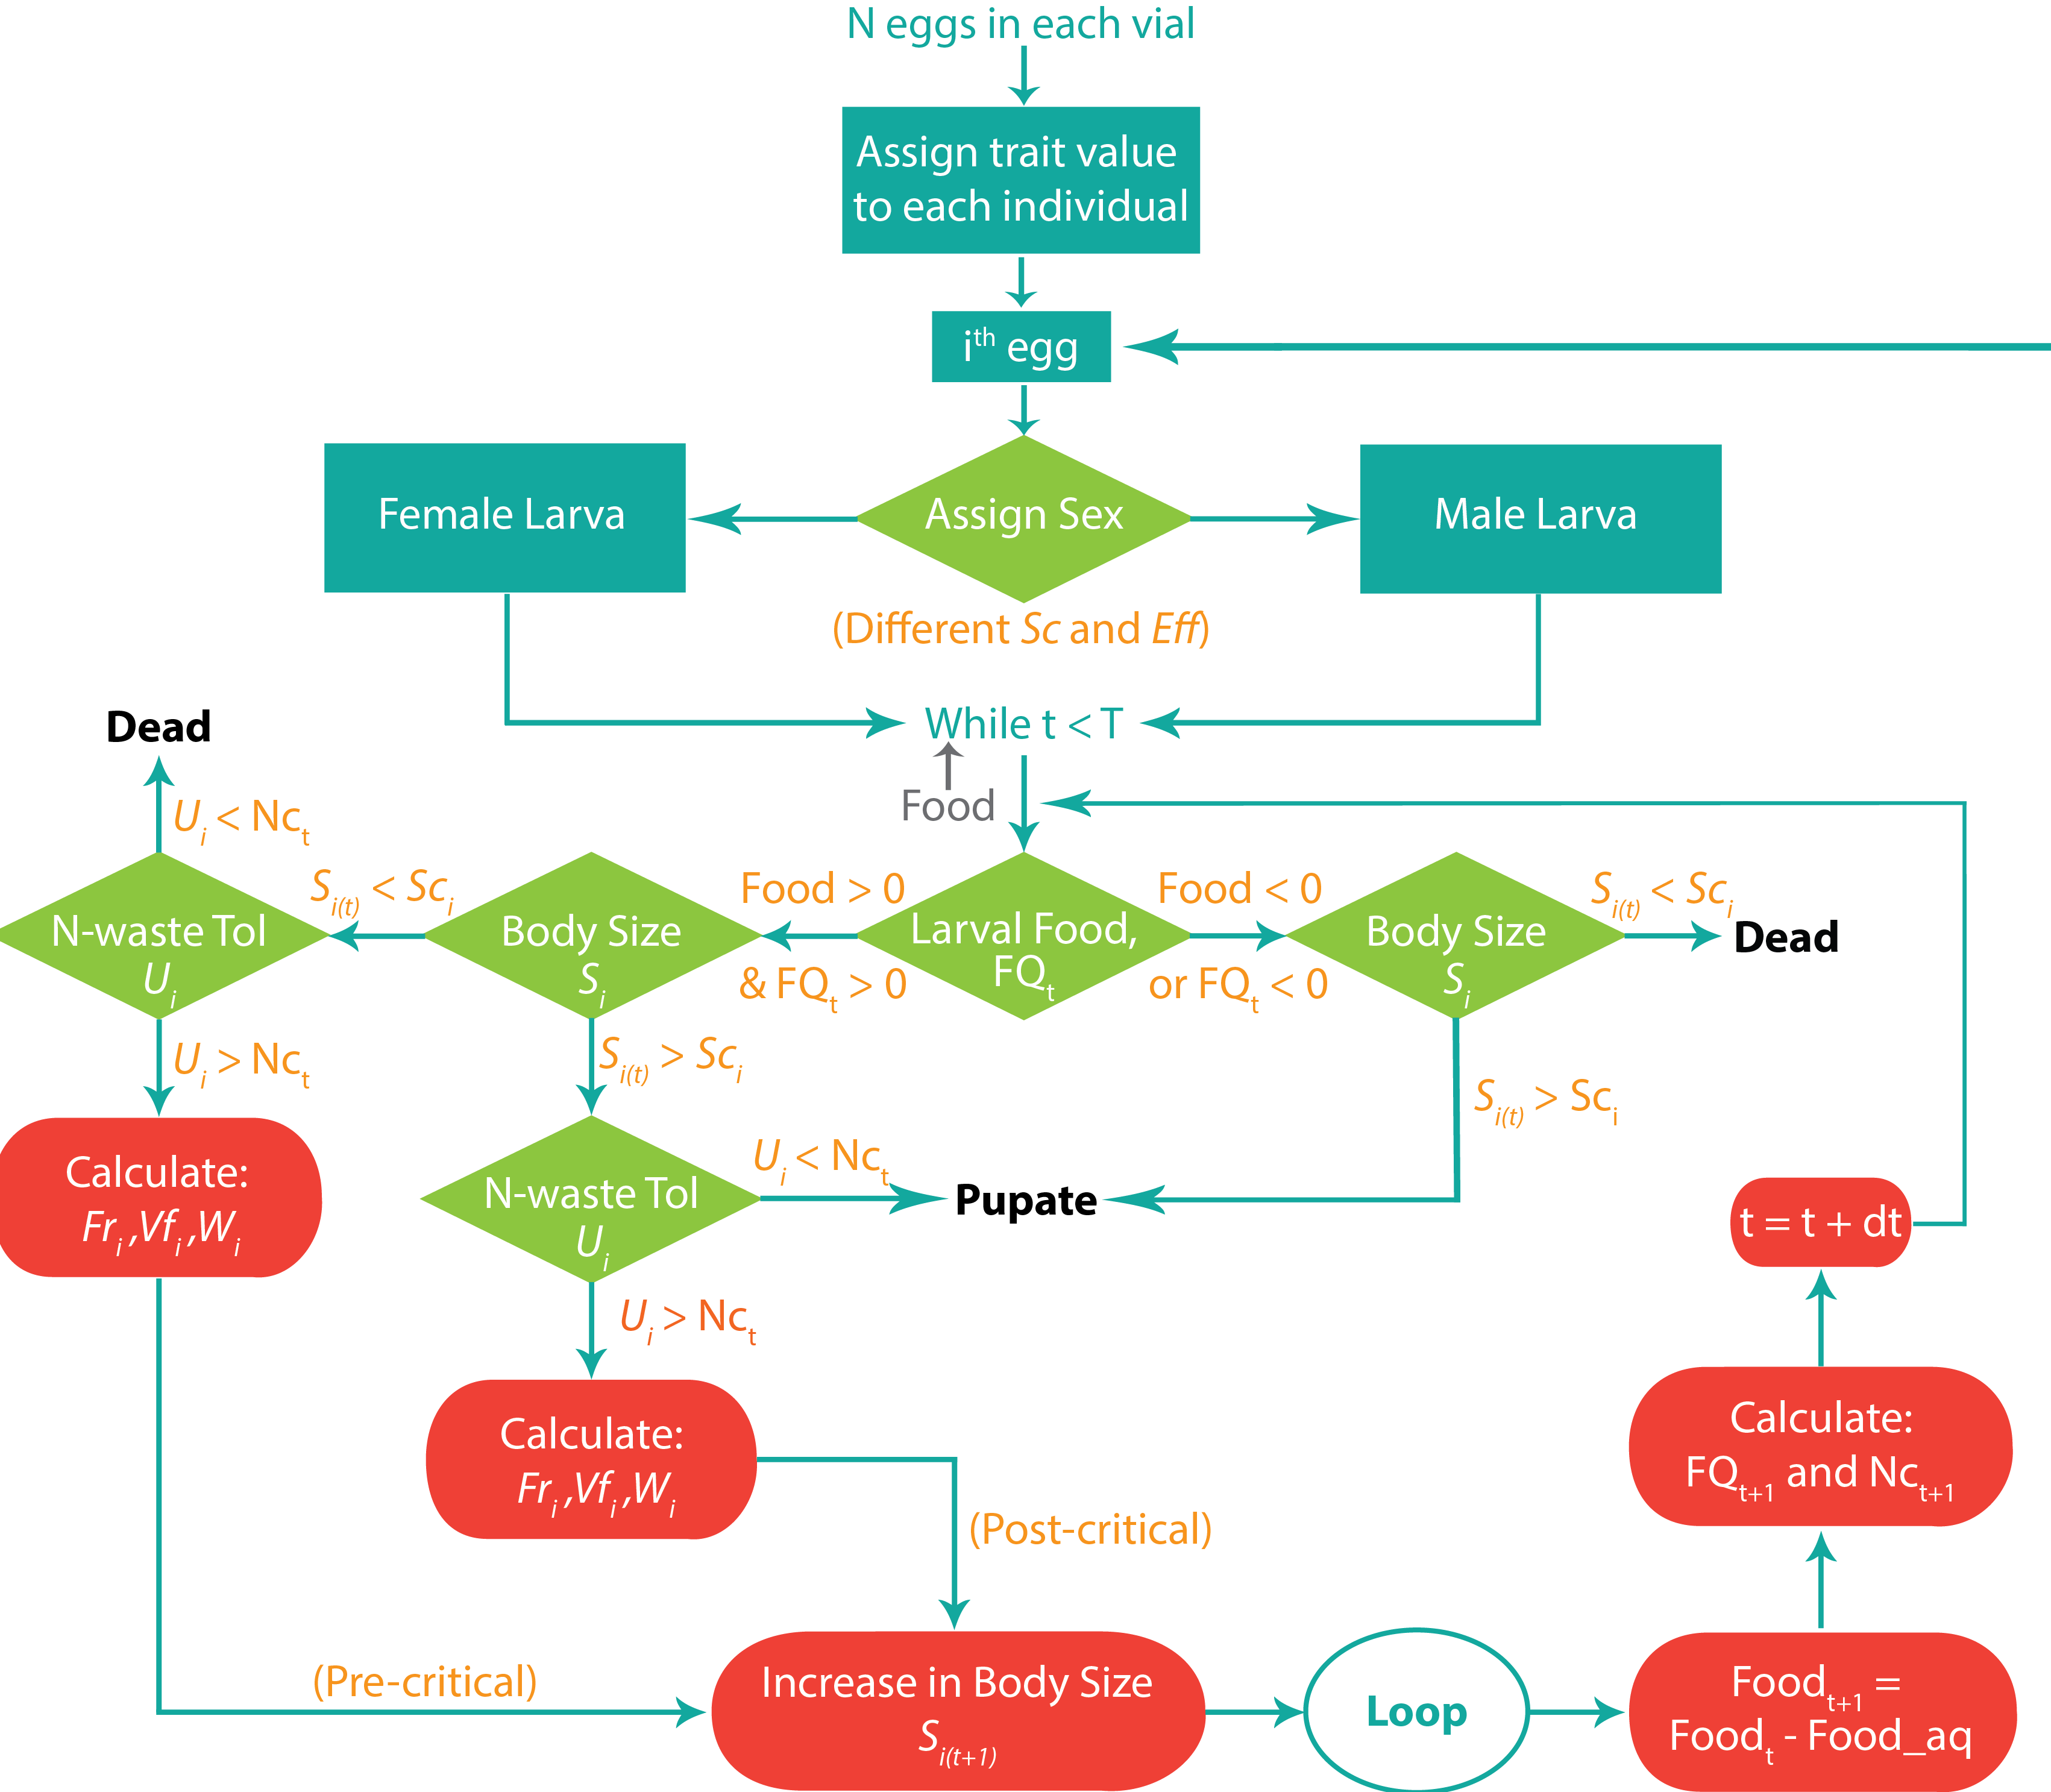
\includegraphics[width=0.8\textwidth]{C2/Figs/larval_model}
  \caption{Flowchart of the larval stage in the model}
  \label{fig:larval_model}
\end{figure}

\noindent Feeding rate stays constant During post-critical stage (see \cite{santosDensityDependentNaturalSelection1997}). During pre-critical growth Volume of food taken in one bite is taken as constant $V_{f}(pre)$ and during post-critical growth it is $V_{f}(post) = 1.5\cdot V_{f}(pre)$. Food consumed by all larvae at time step $t$ is given as:
\[FoodEaten(t) = \sum_{i}food\_eaten_{i}(t) = \sum_{i}Fr_{i}(t)\cdot V_{f}\]
The increase in body size at time $t$ is $S_{i}(t+1)$ and give as:
\[S_{i}(t+1) = S_{i}(t) + food\_eaten_{i}(t)\cdot \epsilon_{i}\cdot FQ_{fb}(t)\]
Here,\\
$\epsilon_{i}$: efficiency to convert food eaten into biomass of $i^{th}$ larvae,\\
$FQ_{fb}(t)$: food quality of the feeding band at time $t$\\ \\
After feeding and utilizing food consumed at given time step, larva produces nitrogenous waste $waste\_prod_{i}(t)$. This affects the total waste produced by all the larvae after feeding:
\[WasteProd(t) = \sum_{i}waste\_prod_{i} = \sum_{i}[food\_eaten_{i}(t)\cdot (1-\epsilon_{i}\cdot FQ(t))]\]
Based on this waste produced, total waste accumulated till time step $t$ in feeding band and diffusion band is calculated considering $k_{d}$ proportion of waste in the feeding band diffuses into diffusion band at each time step.
\[Waste_{fb}(t+1) = Waste_{fb}(t) + (1-k_{d})\cdot WasteProd(t) + \frac{FoodEaten(t)\cdot Waste_{db}}{dband}\]
\[Waste_{db}(t+1) = Waste_{db}(t) + k_{d}\cdot WasteProd(t) - \frac{FoodEaten(t)\cdot Waste_{db}}{dband}\]
Food quality of the feeding band at time step $t$ is:
\[FQ_{fb}(t) = 1 - \frac{Waste_{fb}(t)}{fband}\]
If $FQ_{fb}(t) \leq 0 $, it means that there is no food available to eat and feeding band contains only nitrogenous waste and larvae stop eating.\\
$k_{d}$ is dependent on the food available in the vial and determines whether waste is diffused into the diffusion band. Its values are assigned at each time step as follows:
\begin{enumerate}[i]
  \item $k_{d}$ is a constant $> 0$ ... if $food > (fband+dband)$
  \item $k_{d} = 0$ ... if $food \leq (fband+dband)$
\end{enumerate}
Each larva feeds and increase the body size in each time step based on the conditions for food available ($food$), food quality ($FQ(t)$), critical size ($sc_{i}$) and waste tolerance ($u_{i}$) described in fig~\ref{fig:larval_model}.\\

\noindent Values for all parameters used in the larval stage of the model, are given in table~\ref{tab:trait_value}, table~\ref{tab:scale_param} and table~\ref{tab:food_param}. These values were obtianed by calibrating survivorship, body size and development time results similar to the empirical results in various larval densities \citep{sarangiEcologicalDetailsMediate2018}.
\clearpage
\section{Simulations for Feeding Band Dynamics}
Simulations are performed for trait values in table~\ref{tab:trait_value} to observe the waste build up dynamics and food quality decrease in a food vial with different larval densities during larval feeding.
\subsection{Waste build-up dynamics results}
In fig~\ref{fig:waste}, waste build in the feeding band throughout larval feeding at different larval densities is plotted. At low density i.e. 60 eggs / 6 ml food (MB culture), there is very little nitrogenous waste building up due to diffusion and plenty of food available below the feeding band at all time steps.
\begin{figure}[h]
  \centering
  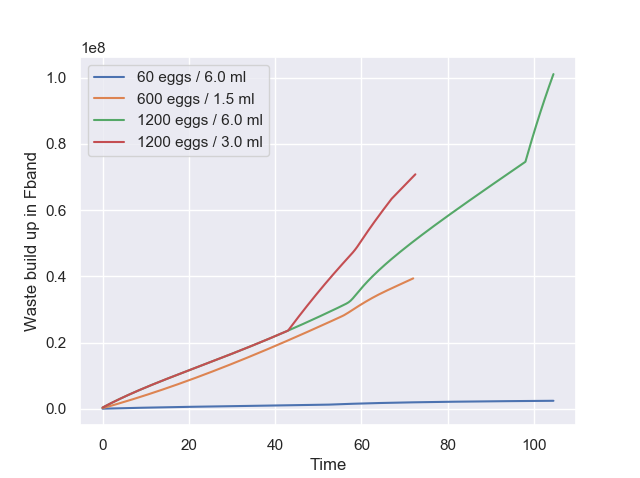
\includegraphics[width=0.8\textwidth]{C2/Figs/waste_build_up}
  \caption{Waste build-up in the feeding band}
  \label{fig:waste}
\end{figure}\\
\noindent High densities of 600 eggs / 1.5 ml food (MCU culture) and 1200 eggs / 3 ml food (CCU culture) show different patterns of waste build up in the feeding band, even though total larval density is equal. In MCU culture vial, there is very little food available below the feeding band, thus diffusion does not occur and waste build in the feeding band increases gradually. In CCU culture vial, waste build-up is almost in same qauntity as in MCU culture in earlier stage, even though effective larval density is double (number of larvae per feeding band). This is due to the availablilty of food below feeding band in CCU culture where waste can diffuse. After approx. $40^{th}$ time step, diffusion stops and waste from diffusion band enters feeding band in more quantity, thus giving a sudden increase in the waste build rate. \\

\noindent LCU culture vial (1200 eggs in 6 ml food) also shows pattern of waste build in the feeding band similar to CCU culture vial, but shows increase in the rate of waste build up approx. after $60^{th}$ time step. This is due to the food is still available below the feeding band. At approx. $100^{th}$ time step in LCU culture vial shows even more increase in the rate of waste build because diffusion band touches the bottom and starts shrinking.\\
\subsection{Food quality dynamics results}
\begin{figure}[h]
  \centering
  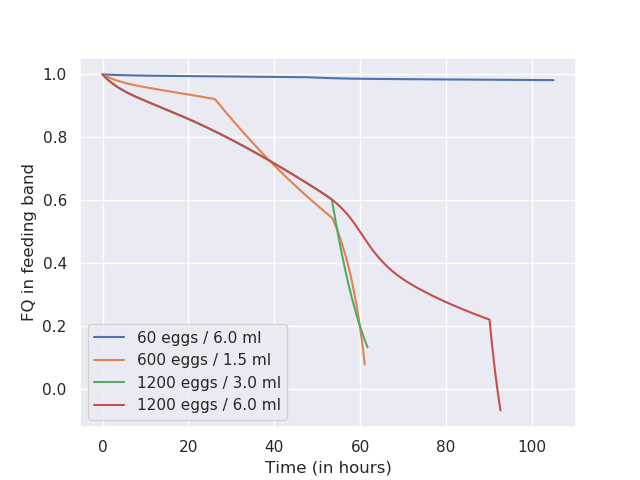
\includegraphics[width=0.8\textwidth]{C2/Figs/fQ}
  \caption{Change in the food quality of feeding band}
  \label{fig:fQ}
\end{figure}
\noindent Fig~\ref{fig:fQ} shows the decrease in the quality of the food present in the feeding band. Food quality being negatively correlated with the amount of waste build-up in the feeding band, it shows patterns similar to waste build-up during larval growth in all crowding condtions. Since food quality affects body size increment at each time step. Body size increment between $40^{th}$ and $60^{th}$ time step is completely different in MCU and CCU cultures even though there larval density is equal. In LCU culture, decrease in food quality is simlar to CCU culture till ~$60^{th}$ time step but later decreases gradually unlike CCU. This gradual decrease is due to gradual waste diffusion into the available food below the feeding and diffusion band. Once diffusion band hits the bottom at ~$90^{th}$ time step, food quality decreases rapidly.
\pagebreak
